\documentclass[12pt]{article}
\usepackage[spanish]{babel}
\usepackage[utf8]{inputenc}     % Para que acepte acentos y ñ directamente
\usepackage[T1]{fontenc}        % Mejor manejo de caracteres acentuados
\usepackage{geometry}
\geometry{a4paper, margin=1in}
\usepackage{graphicx}
\usepackage{xcolor}
\usepackage{titlesec}
\usepackage{parskip}
\usepackage{multicol}
\usepackage{cite}
\usepackage{hyperref}           % Para hipervínculos en PDF
\usepackage{url}
\hypersetup{
  colorlinks=true,
  linkcolor=blue,
  citecolor=blue,
  urlcolor=blue
}
\definecolor{highlight}{RGB}{255, 255, 0}

\titleformat{\section}{\normalfont\Large\bfseries}{\thesection}{1em}{}
\titleformat{\subsection}{\normalfont\large\bfseries}{\thesubsection}{1em}{}

\begin{document}

% Logos
\begin{minipage}{0.45\textwidth}
    
\includegraphics[width=0.4\textwidth]{inFiles/Figures/epnLogo.jpg}
\end{minipage}
\hfill
\begin{minipage}{0.45\textwidth}
    \raggedleft
    
\includegraphics[width=0.4\textwidth]{inFiles/Figures/FIS_logo.jpg}
\end{minipage}

\vspace{0.5cm}

% Títulos principales
\begin{center}
    \textbf{ESCUELA POLITÉCNICA NACIONAL}\\[0.2cm]
    \textbf{FACULTAD DE INGENIERÍA DE SISTEMAS}\\[0.2cm]
    \textbf{INGENIERÍA {\textbf{EN COMPUTACION}}}
\end{center}

\vspace{0.5cm}
\hrule
\vspace{0.5cm}

% Datos principales
\noindent\textbf{PERÍODO ACADÉMICO:} 2025-A\\[0.2cm]
\noindent\textbf{ASIGNATURA:} ICCD412 Métodos Numéricos \hfill \textbf{GRUPO:} GR2\\[0.2cm]
\noindent\textbf{TIPO DE INSTRUMENTO:} {Practica 3}\\[0.2cm]
\noindent\textbf{FECHA DE ENTREGA LÍMITE:}{07/05/2025}\\[0.2cm]
\noindent\textbf{ALUMNO:} {Lema Luis}

\vspace{0.5cm}
\hrule
\vspace{1cm}


% Secciones
\section*{TEMA}
{Tipos de errores}

\vspace{0.5cm}

\section*{OBJETIVOS}
\begin{itemize}
    \item Comprender el fundamento teórico del método de la bisección y su aplicabilidad en la resolución de ecuaciones.
    \item Implementar el método de bisección en problemas del mundo real como el cálculo del volumen en un abrevadero semicircular y la determinación del tiempo de caída de un objeto bajo resistencia del aire.
    \item Evaluar la precisión de los resultados obtenidos mediante una cota de error predefinida, asegurando confiabilidad en la solución.
    \item Desarrollar pensamiento analítico a través del análisis iterativo de soluciones aproximadas y el comportamiento de funciones no lineales.
\end{itemize}

\vspace{0.5cm}

\section*{MARCO TEÓRICO}

{Esta herramienta se vuelve especialmente útil cuando no se puede encontrar una solución exacta de manera algebra
  ica, lo cual es común en problemas reales de física e ingeniería. Aunque su velocidad de convergencia es menor 
  comparada con otros métodos como el de Newton-Raphson o el de la secante, el método de la bisección destaca por su estabilidad 
  y su facilidad de implementación, siendo ideal para introducir a los estudiantes en el análisis de métodos numéricos.} \cite{chapra}

  {La forma en que opera este método consiste en dividir repetidamente el intervalo inicial en dos subintervalos, 
  seleccionando aquel en el que la función continúa cambiando de signo. Este proceso se repite hasta que se cumple un criterio 
  de tolerancia definido previamente, lo cual garantiza una aproximación aceptable de la raíz con el nivel de precisión deseado.} \cite{chapra}
 
   {Desde un enfoque pedagógico, el método permite a los estudiantes familiarizarse con conceptos como el error absoluto, 
   el número de iteraciones necesarias y la convergencia de los métodos numéricos. Además, ofrece una oportunidad para reflexionar
    sobre la importancia del análisis de errores, ya que tanto los errores de redondeo como los de truncamiento pueden influir en
     la calidad del resultado final.
   } \cite{mathews}

   {En conclusión, aunque el método de la bisección no es el más eficiente desde el punto de vista computacional, 
   su seguridad y facilidad de aplicación lo convierten en una herramienta indispensable para el desarrollo del pensamiento lógico
    y numérico, especialmente en etapas formativas.

   } \cite{fisicalabErrores}

\vspace{0.5cm}

\section*{DESARROLLO}
\begin{minipage}{0.95\textwidth}
    \raggedleft
    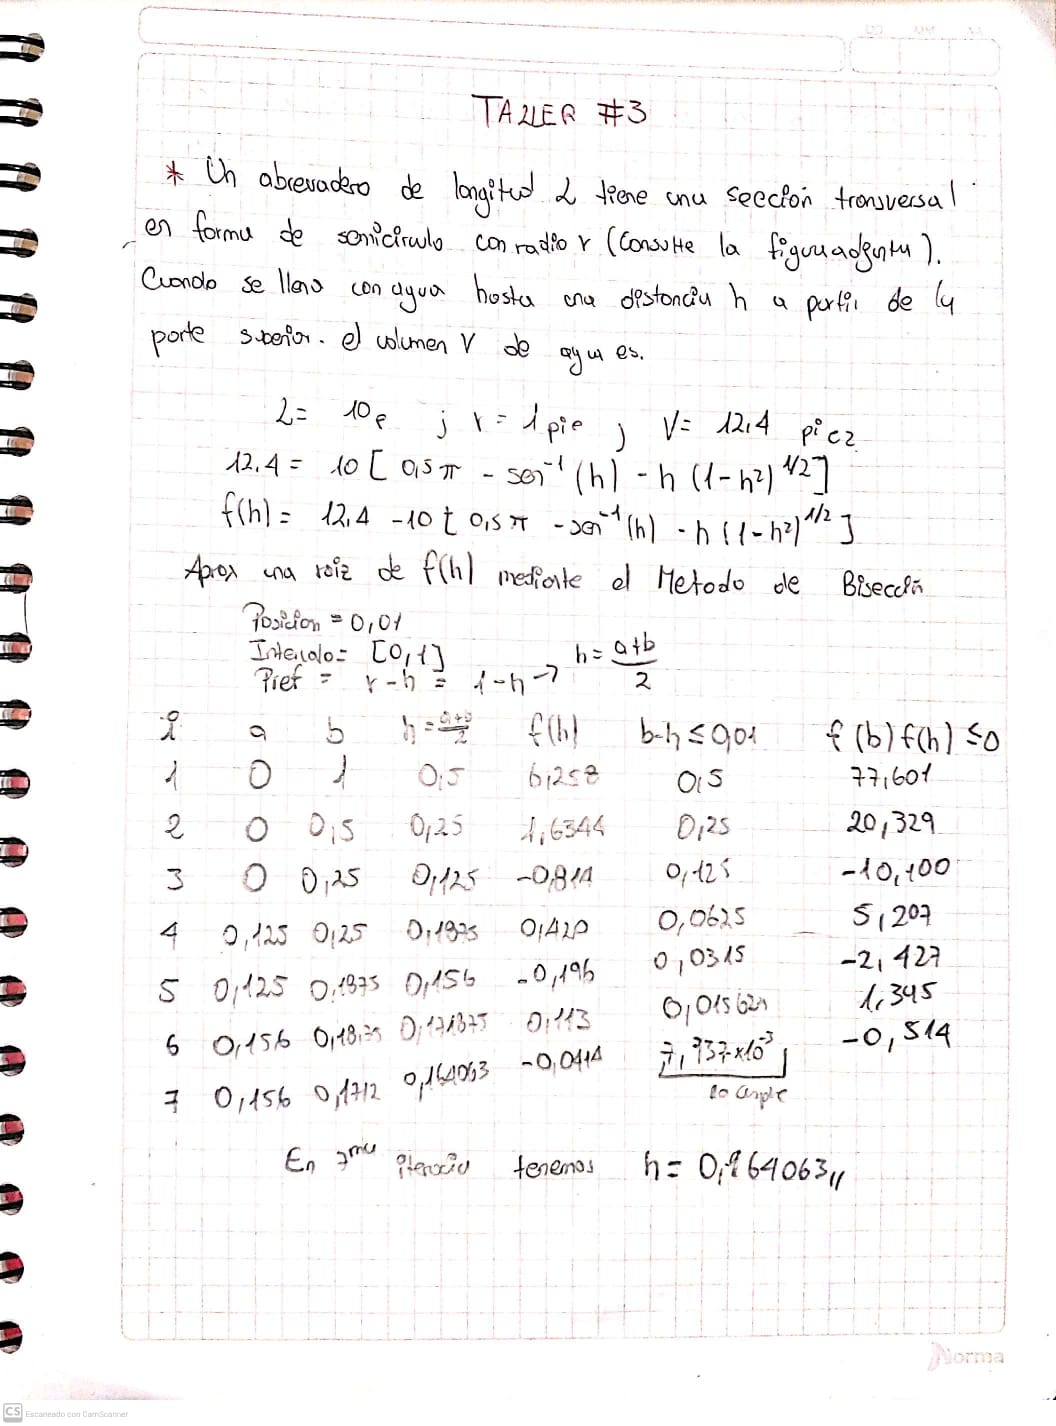
\includegraphics[width=0.95\textwidth]{inFiles/Figures/ej1.jpeg}
\end{minipage}

\vspace{0.5cm}

\begin{minipage}{0.95\textwidth}
    \raggedleft
    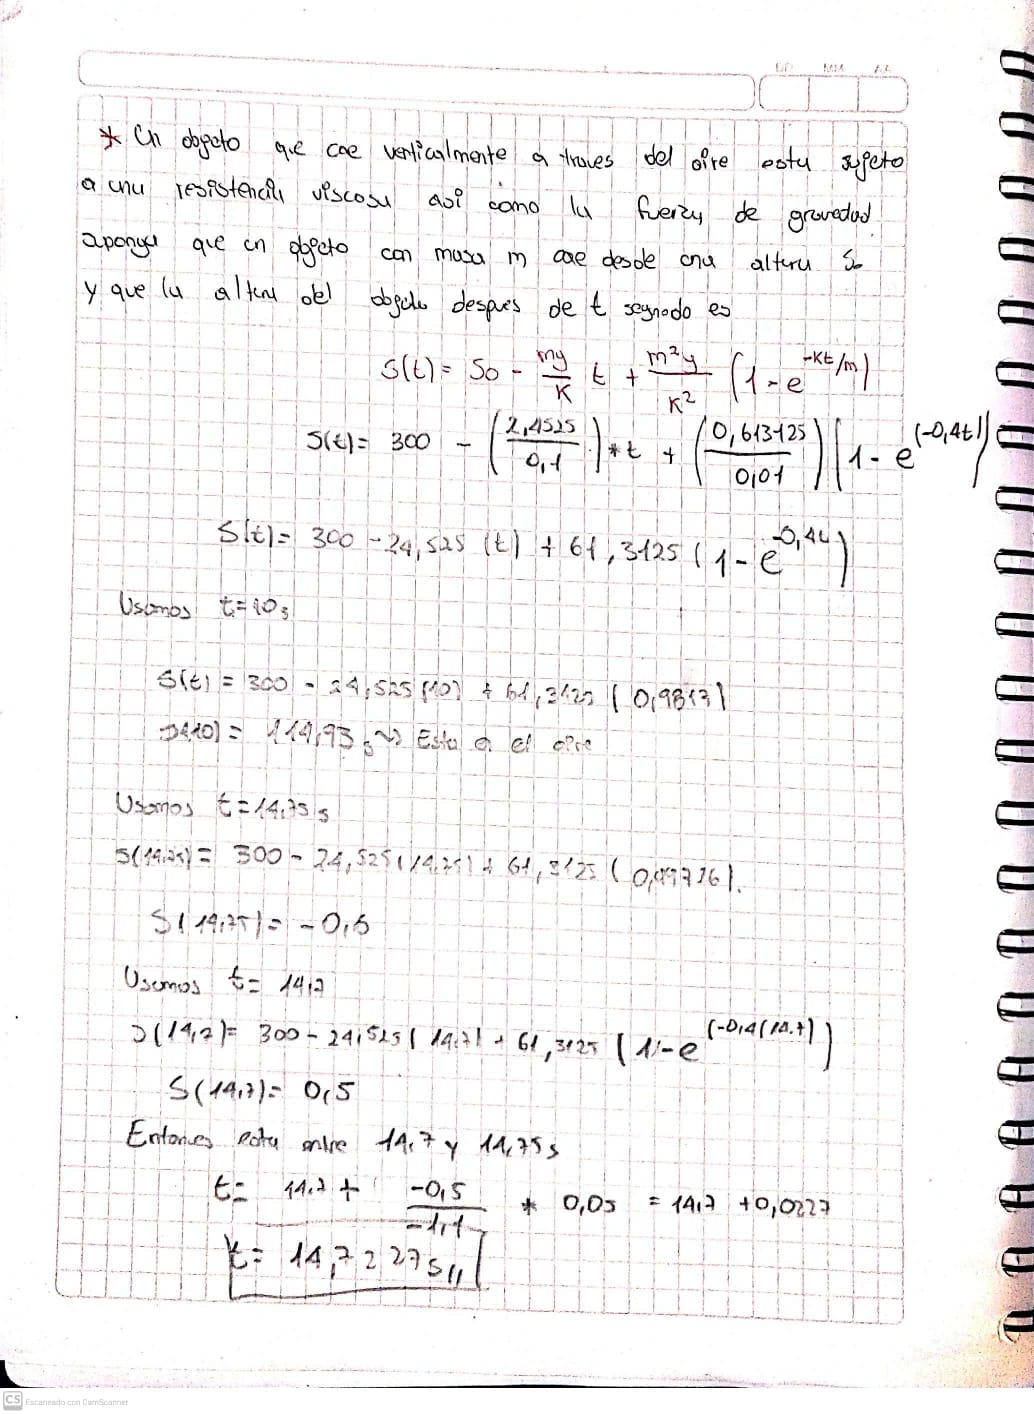
\includegraphics[width=0.95\textwidth]{inFiles/Figures/ej2.jpeg}
\end{minipage}

\vspace{0.5cm}

\begin{minipage}{0.95\textwidth}
    \raggedleft
    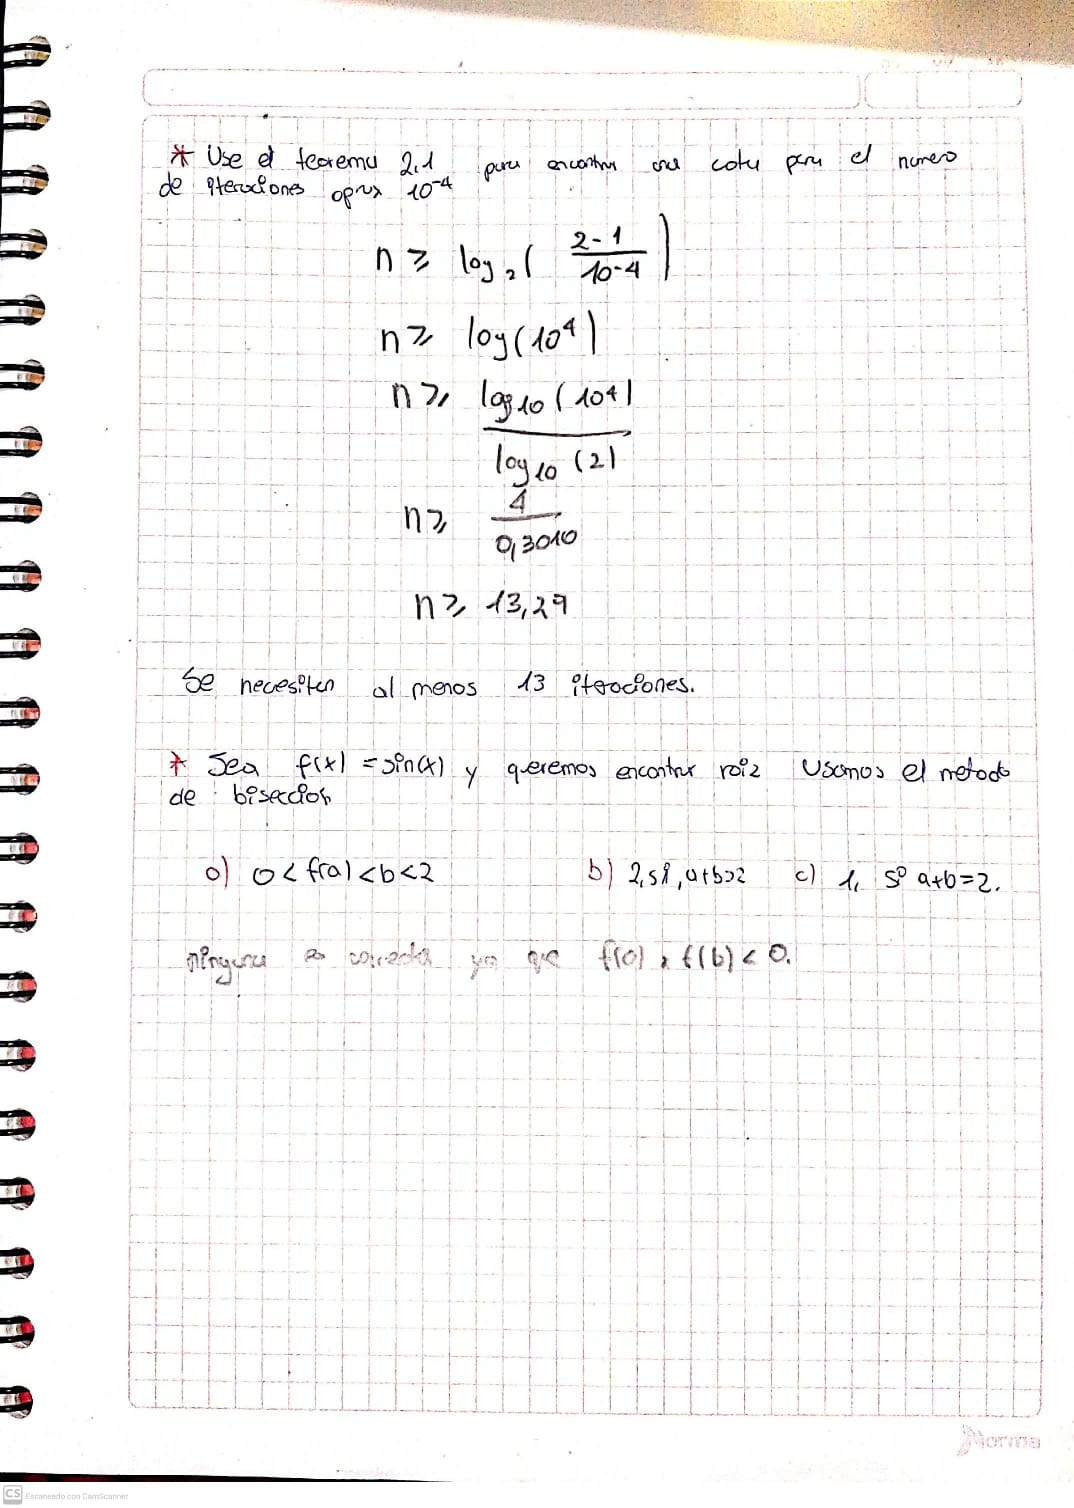
\includegraphics[width=0.95\textwidth]{inFiles/Figures/ej3.jpeg}
\end{minipage}

\vspace{3cm}


\section*{CONCLUSIONES}
\begin{itemize}
    \item El método de la bisección demostró ser una herramienta efectiva y confiable para encontrar raíces de funciones continuas, especialmente en contextos donde no se dispone de soluciones analíticas exactas.

    \item Su simplicidad algorítmica lo convierte en un método ideal para la formación académica, permitiendo a los estudiantes comprender de manera clara los fundamentos de los métodos numéricos y el comportamiento de funciones no lineales.

    \item Se comprobó que, bajo condiciones básicas como la continuidad de la función y el cambio de signo en un intervalo, el método garantiza convergencia hacia una solución con la precisión deseada.

    \item La correcta elección del intervalo inicial y la tolerancia de error fueron aspectos fundamentales para lograr resultados precisos y eficientes.

    \item A través de la aplicación práctica del método en problemas reales de física y geometría, se fortalecieron habilidades como el análisis crítico, la lógica matemática y la interpretación de resultados numéricos.

    \item El ejercicio permitió también reflexionar sobre la importancia del análisis de errores en los métodos numéricos, como los errores de redondeo y truncamiento, que pueden influir significativamente en los resultados obtenidos.
\end{itemize}


\vspace{0.5cm}

\section*{RECOMENDACIONES}
\begin{enumerate}
    \item  Es crucial garantizar que el intervalo inicial seleccionado contenga un cambio de signo en la función evaluada. Esto garantiza la existencia de una raíz y evita errores lógicos durante la ejecución del método.
    
    \item  Se debe seleccionar una tolerancia acorde al problema. Tolerancias muy bajas aumentan el número de iteraciones, lo que puede incrementar el costo computacional sin aportar mejoras significativas en la práctica.
    
    \item  Aunque el método de la bisección no es el más eficiente para funciones con múltiples raíces o para situaciones donde se requiera una rápida convergencia, su claridad y estabilidad lo convierten en una herramienta idónea para la formación de criterio numérico en los estudiantes.
    
    \item En escenarios reales de ingeniería o física, se recomienda emplear el método de la bisección como una etapa preliminar o de validación para métodos más avanzados como Newton-Raphson o la secante, especialmente en casos donde no se conoce bien el comportamiento de la función.
\end{enumerate}

\vspace{0.5cm}


\renewcommand{\refname}{\MakeUppercase{REFERENCIAS}}
\bibliographystyle{IEEEtran}
\bibliography{inFiles/References/references.bib}
\end{document}
